\section{Statistische Grundlagen}
Zunächst wiederholen wir ein paar Grundlagen aus der Statistik.

\subsection{Beschaffenheit von Daten}
Daten können in verschiedenen Kategorien vorliegen:
\begin{itemize}
	\item \textbf{Nominal}: Hier herrscht keine natürliche Ordnung der Werte (z.B. Name, Farbe, ...)
	\item \textbf{Ordinal}: Eine Anordnung ist möglich. Es kann jedoch nicht ohne Weiteres eine Metrik angelegt werden (z.B.  ist nicht quantifiziert, um wie viel sich groß und gigantisch unterscheiden)
	\item \textbf{Metrisch-diskret}: Es existiert eine endliche Anzahl an Werten, auf die eine Metrik angewandt werden kann (z.B. \({n\in \mathbb{N}\ |\ n \in [0,100]}\))
	\item \textbf{Metrisch-kontinuierlich}: Es existieren unendlich viele Werte, auf die eine Metrik angewandt werden kann (z.B. \({n\in \mathbb{R}\ |\ n \in [0,100]}\))
\end{itemize}
Weiter können die Datensätze auch unterschiedlich komplex sein. Die kann sich unter anderem in der \textbf{Dimensionalität} der Daten widerspiegeln. So haben offensichtlich die Datensätze einer einfachen Namensliste eine geringere Dimension als die  in den Kundendatenbanken einer großen Firma.

Betrachten wir metrisch skalierte Daten, so gilt für eine Metrik d und Domäne M:
\begin{align*}
	&\forall p,q,r \in M:&\\
	\\
	&Symmetrie &d(p,q)=d(q,p)\\
	&Definitheit &d(p,q)=0\Leftrightarrow p = q\\
	&Dreiecksungleichung &d(p,r)\leq d(p,q)+d(q,r)\\
\end{align*}
Metrik bezeichnet hierbei eine Funktion, die den Abstand zweier Punkte im Raum beschreibt.

\subsection{Einfache deskriptive Statistik}
Im Folgenden betrachten wir einfache Methoden zur Beschreibung von Daten, um diese besser verstehen zu können. Dafür dienen vor allem so genannte \textbf{Aggregate}. Sie vereinen \textit{alle Werte} eines Attributes und berechnen daraus einen \textit{einzigen} skalaren Wert. In Standard-SQL werden folgende Funktionen verwendet: 
\begin{itemize}
	\item COUNT() - Zählt die Anzahl
	\item SUM() - Bildet die Summe
	\item MIN() - Gibt das Minimum aus
	\item MAX() - Gibt das Maximum aus
	\item AVG() - Berechnet das arithmetische Mittel
\end{itemize}
In spezialisierteren SQL-Versionen gibt es weitere Aggregatsfunktionen (z.B. für die Bereiche Statistik, Physik, etc.). Manche dieser Aggregate haben den Vorteil, dass sie sich in ihrer Ausführung parallelisieren lassen, z.B. kann für die MIN()-Funktion der Datenbestand in kleinere Bestände aufgeteilt werden, aus denen jeweils das Minimum berechnet wird, woraufhin in einem zweiten Schritt das Minumim der Minima berechnet wird.
Aufgrund dieser Eigenschaften lassen sich die Aggregate klassifizieren (\(F\) bezeichne die Aggregatsfunktion):
\begin{itemize}
	\item \textbf{distributiv}: Formal gibt es eine Funktion \(G\), so dass \(F(\{X_{i,j}\}) = G(\{F(\{X_{i,j}| i = 1, ..., I\}) | j = 1, ..., J\})\) gilt. Auf Deutsch: F wird erst auf Teilmengen ausgeführt, dann G auf der Ergebnismenge. Hierbei ist \(I \in \mathbb{N}\) die Mächtigkeit der Teilmengen und \(J\in\mathbb{N}\) ihre Anzahl (es ist nicht zwingend notwendig, dass alle Teilmengen auch tatsächlich die gleiche Mächtigkeit haben).
	\item \textbf{algebraisch}: Formal gibt es eine Funktion \(G\), die \(M\)-Tupel liefert und \(H\), so dass \(F(\{X_{i,j}\}) = H(\{G(\{X_{i,j}| i = 1, ..., I\}) | j = 1, ..., J\})\) gilt. Auf Deutsch: Die Definition entspricht der distributiver Aggregate, jedoch hat man hier die Freiheit, in der inneren Klammer eine Funktion anzuwenden, die nicht die Ausgangsaggregatfunktion \(F\) ist. So könnte man z.B. AVG() folgendermaßen formalisieren:
	\begin{align*}
		G &: \text{Menge von } \mathbb{R} \rightarrow (\mathbb{R},\mathbb{N}),\ S \mapsto a:= (\sum_{x\in S} x, |S|) \\
		H &: \text{Menge von } (\mathbb{R},\mathbb{N}) \rightarrow \mathbb{R},\ a \mapsto \frac{\sum\nolimits_{a\in A} a.first}{\sum\nolimits_{a\in A}a.second}
	\end{align*}
	\item \textbf{holistisch}: Holistische Aggregate sind all jene, die weder distributiv noch algebraisch sind. Man kann das Problem also nicht in Teilprobleme zerlegen, z.B. bei median() oder häufigsterWert(). \textbf{Definition aus der Vorlesung}: Man kann keine Beschränkung des Speicherbedarfs für Sub-Aggregate angeben.
\end{itemize}
Offensichtlich sind distributive bzw. algebraische Aggregate aufgrund ihrer Parallelisierungsmöglichkeiten effizienter in ihrer Berechnung.

\noindent Eine weitere vorteilhafte Eigenschaft, die eine Aggregatsfunktion haben kann, heißt \textbf{"'Self-Maintainable"'}. Self-Maintainable Aggregatsfunktionen können nach einer Änderung der Daten ihren neuen Wert aus ihrem alten Wert und der Änderung berechnen, z.B. SUM(). Änderungen bedeutet in diesem Fall Einfügen oder Löschen von Daten.

\subsection{Qualifizierung der Tendenz insgesamt}
Als nächstes geht es um Kennzahlen, die etwas über die Tendenz in unseren Daten aussagen. Die bekannteste ist das \textbf{arithmetische Mittel}
\[\bar{x}= \frac{1}{n} \sum_{i=1}^n x_i\ .\]
Dieses kann man auch weiter verfeinern zum \textbf{gewichteten arithmetischen Mittel}
\[\bar{x}_w = \frac{\sum_{i=1}^n w_i * x_i}{\sum_{i=1}^n w_i}\ .\]
Anschaulich beschrieben, wird jedes \(x_i\) mit einem prozentualem Wert multipliziert, wobei sich diese Gewichte zu 1 aufaddieren.
Laut obiger Klassifikation lassen sich diese Kennzahlen als \textit{algebraisch} einstufen. Des Weiteren sind sie nur auf numerische Daten anwendbar.
Wenn es um die Mitte unseres Wertebereiches geht, kann das sogar ein Grundschüler ausrechnen:
\[midrange = \frac{max - min}{2}\]
Auch \textit{midrange} kann nur auf numerische Daten angewandt werden.

Der \textbf{Median} gibt bei sortierter Anordnung den Wert an, der in der Mitte liegt:
\[
x_{med} = 
\begin{cases}
	x_{\frac{n+1}{2}} &\quad \text{für } n \text{ ungerade}\\
	\frac{1}{2}(x_{n/2} + x_{n/2+1}) &\quad \text{für } n \text{ gerade}\
\end{cases}
\]
Der Median lässt sich auf numerische und ordinale Daten anwenden und ist als \textit{holistisch} einzustufen.

Der \textbf{Modus} gibt den Wert an, der im Datenbestand am häufigsten vorkommt. Wenn jeder Wert im Datenbestand nur ein \emph{einziges} Mal auftaucht, ist der Modus nicht definiert. Dies führt bei kontinuierlichen Daten schnell zu Problemen.

\noindent Beim Modus muss beachtet werden, dass evtl. wichtige Informationen über unsere Daten ignoriert werden können, z.B. weitere Peaks bei multimodalen Verteilungen.

\subsection{Quantifizierung der Streuung der Daten}
\textbf{Quantile} sind Lagemaße, die einen Schwellenwert in unseren Daten beschreiben, d.h. ein bestimmter Anteil ist kleiner als das Quantil, der Rest ist größer. Besondere Quantile sind die \textbf{Quartile}: Das 0.25-Quartil \(Q_{0.25}\) bzw. \(Q_1\) gibt den Wert an, für den 25\% der Werte kleiner oder gleich und 75\% der Werte größer oder gleich \(Q_1\) sind. Analog wird \(Q_{0.75}\) bzw. \(Q_3\) definiert. Es gilt: \(Q_2 = Q_{0.5} = x_{med}\). Mit diesen Quartilen lässt sich der so genannte \textbf{Inter-Quartils-Abstand} definieren als \(IQR = Q_3 - Q_1\). Als \textbf{Ausreißer} bezeichnet man Werte, die mehr als \(1,5 \times IQR\) von \(Q_1\) nach unten oder \(Q_3\) nach oben abweichen.

Weitere wichtige Streumaße sind \textbf{Varianz} und \textbf{Standardabweichung}:
\begin{align*}
	\sigma^{2} &= \frac{1}{n-1}\sum\limits_{i=1}^n (x_i -\bar{x})^2 \\
	\sigma &= \sqrt{\sigma^{2}} \\
\end{align*}

\subsection{Boxplots}
Wir halten uns kurz.

\noindent Die Daten in Abb.~\ref{fig:boxplot} sind als Box repräsentiert. Die Ränder der Box sind \(Q_1\) bzw. \(Q_3\), womit die Höhe der Box dem \(IQR\) entspricht. Innerhalb der Box ist \(x_{med}\) explizit eingezeichnet. Das Minimum und Maximum sind als "'whiskers"' eingezeichnet.
\begin{figure}[ht]
	\centering
	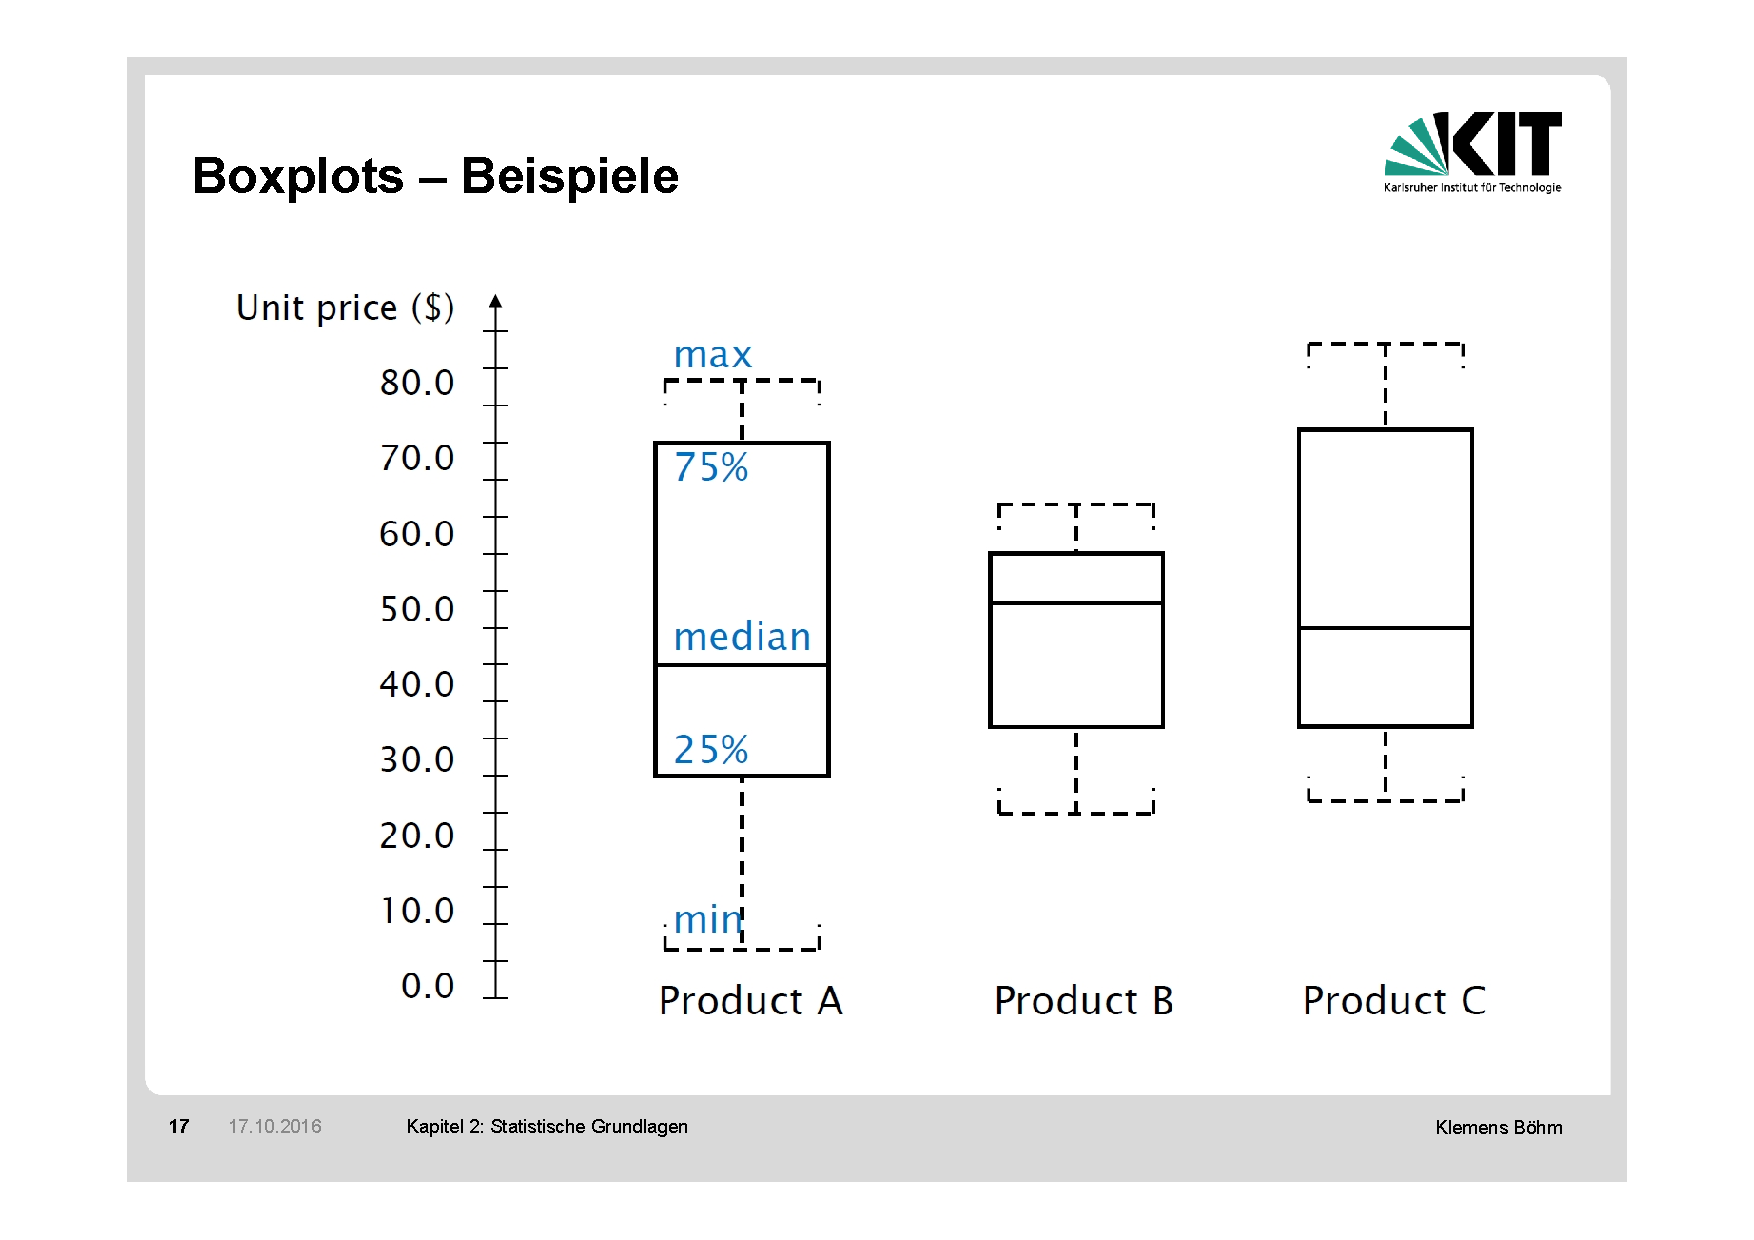
\includegraphics[width=0.625\textwidth]{Figures/boxplot}
	\caption[Boxplot Beispiel]{Beispiel eines Boxplots \footnotemark}
	\label{fig:boxplot}
\end{figure}
\footnotetext{2. Foliensatz, S.17, Analysetechniken für große Datenbestände, Prof. Dr.-Ing. Klemens Böhm}

\subsection{Histogramme}
\textbf{Histogramme} zeigen die Häufigkeit, mit der einzelne Werte auftreten. Falls nahezu bzw. alle Werte unterschiedlich sind, hat man jedoch mit einem Histogramm nichts gewonnen. Deswegen werden die Daten in Klassen bzw. "'Buckets"' unterteilt. Dies stellt im Allgemeinen eine recht gute Approximation dar. Wählt man die Partitionierung der Art, dass alle Klassen gleich breit sind, erhalten wir ein \textit{Equi-Width}-Histogramm, Abb.~\ref{fig:equiWidth}.

\begin{figure}[ht]
	\centering
	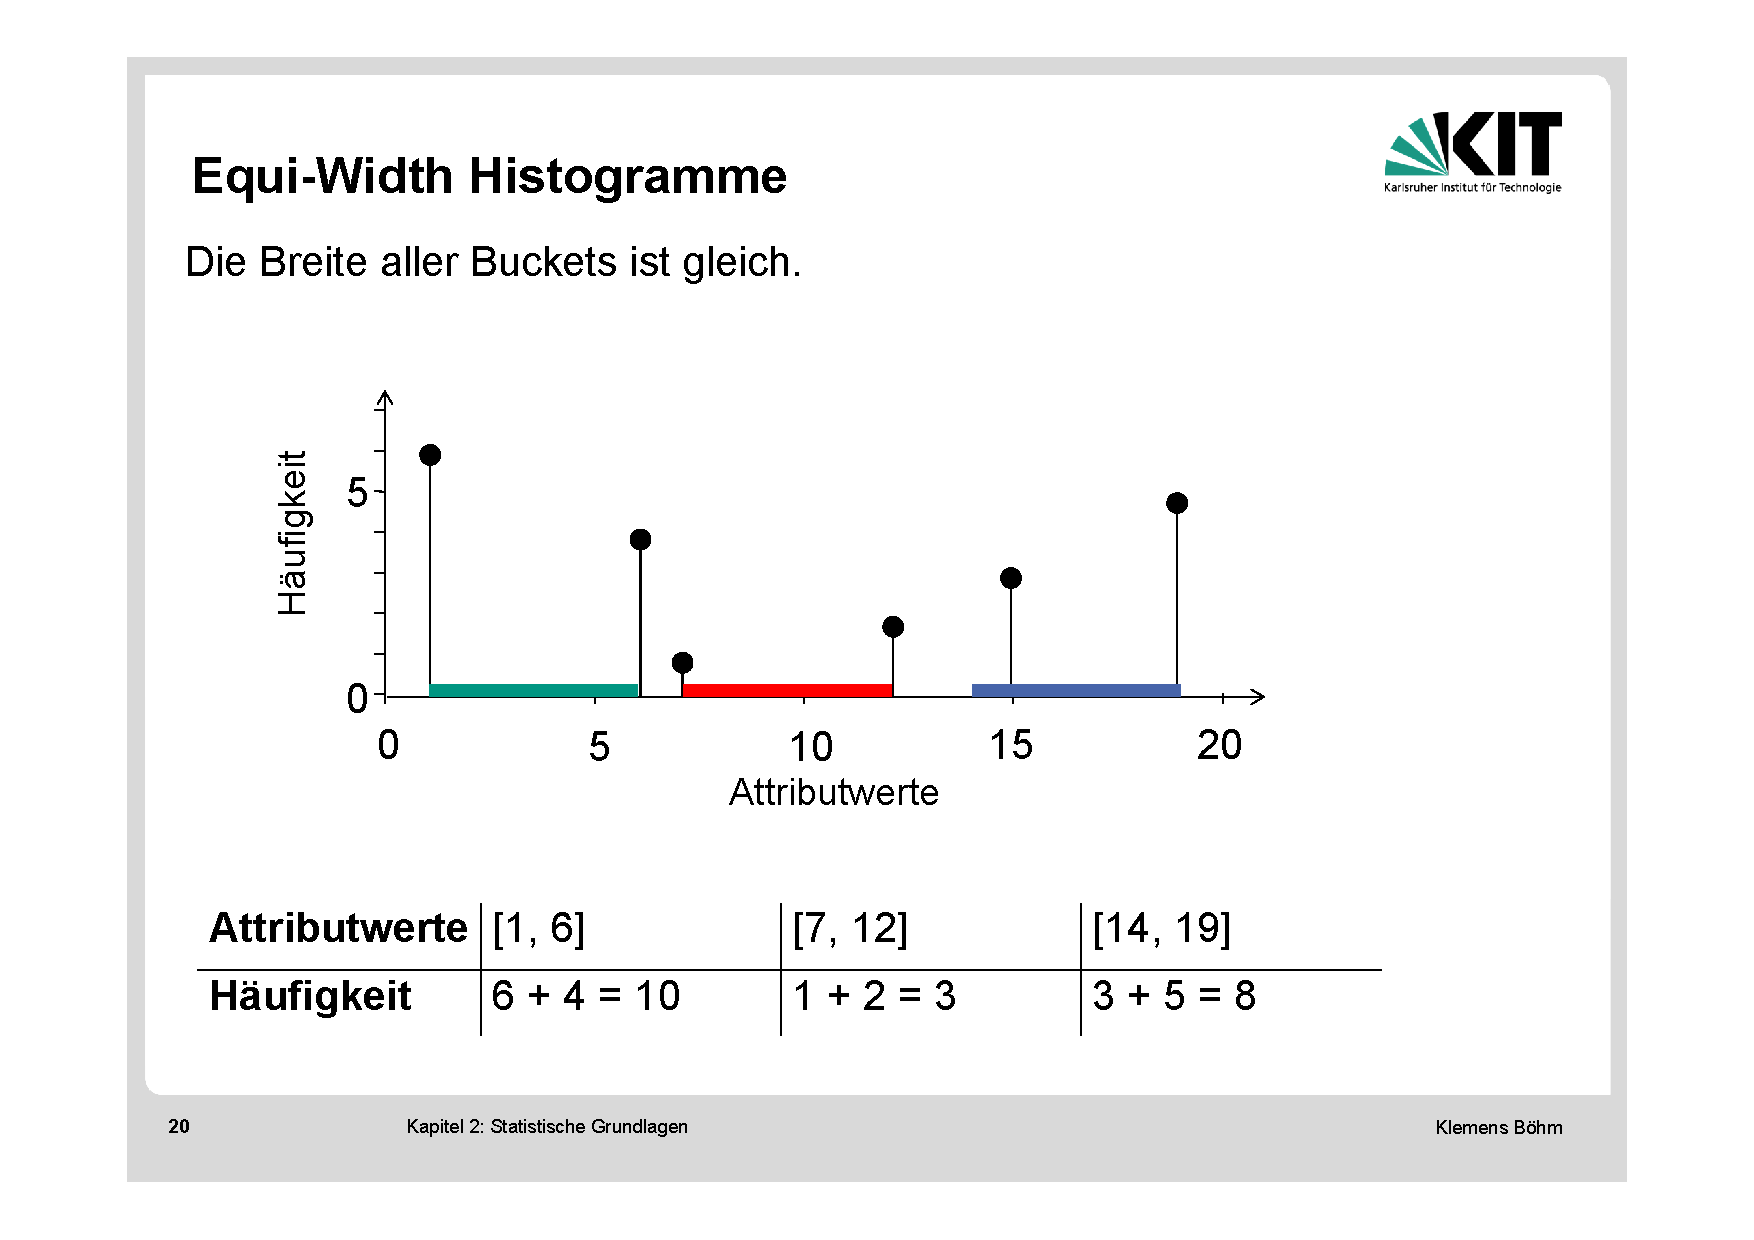
\includegraphics[width=0.625\textwidth]{Figures/equiWidth}
	\caption[Equi-Width Beispiel]{Beispiel eines Equi-Width-Histogramms \footnotemark}
	\label{fig:equiWidth}
\end{figure}
\footnotetext{2. Foliensatz, S.20, Analysetechniken für große Datenbestände, Prof. Dr.-Ing. Klemens Böhm}

\noindent Wählt man jedoch die Klassen so, dass alle gleich viele Elemente enthalten, so ergibt sich ein \textit{Equi-Depth}-Histogramm, Abb.~\ref{fig:equiDepth}.

\begin{figure}[ht]
	\centering
	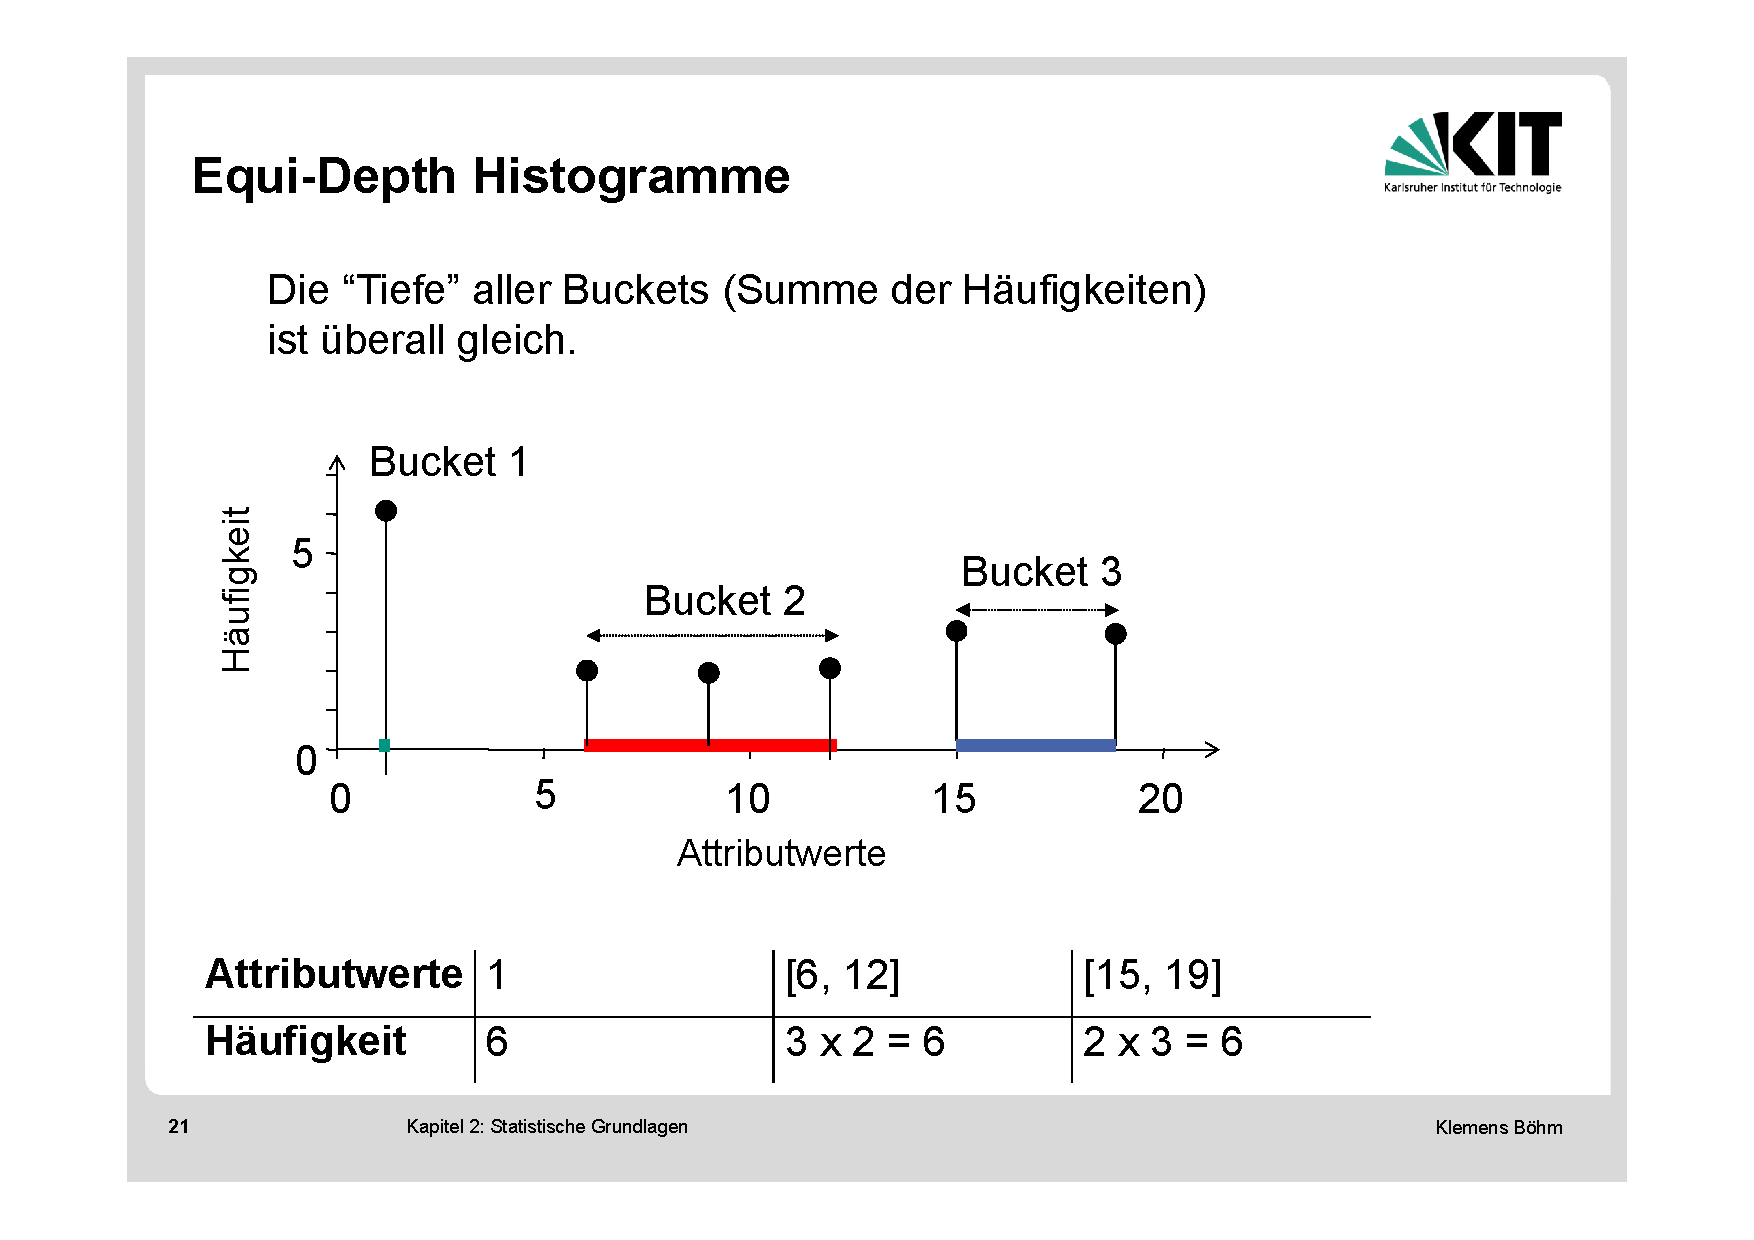
\includegraphics[width=0.625\textwidth]{Figures/equiDepth}
	\caption[Equi-Width Beispiel]{Beispiel eines Equi-Depth-Histogramms \footnotemark}
	\label{fig:equiDepth}
\end{figure}
\footnotetext{2. Foliensatz, S.21, Analysetechniken für große Datenbestände, Prof. Dr.-Ing. Klemens Böhm}

Probleme ergeben sich für Histogramme bei höher dimensionalen Datenbeständen. In den Beispielen der Abb.~\ref{fig:equiWidth} und~\ref{fig:equiDepth} handelt es sich um 1-dimensionale Daten. Diese können leicht klassiert werden. Wie aber sollen z.B. 4-dimensionale Daten gleichmäßig auf Buckets verteilt werden? Außerdem legt man zu Beginn fest, wie groß die Partitionierung ausfällt, womit bei späteren Schätzungen, die auf diesen Histogrammen basieren, nicht weiter mit der Genauigkeit variiert werden kann. Insgesamt ist die Genauigkeit der Approximation durch ein Histogramm in hohem Maße abhängig von der richtigen Wahl der Partitionierung.

\subsection{Entropie}
Die \textbf{Entropie} einer Menge gibt an, wie zufällig die Daten in ihr verteilt sind, d.h. die Entropie dient als Maß für die Unordnung und ist definiert als
\[
	E(S)=-\sum\limits_{j\in S} p_j \cdot \log{p_j}.
\]
Hierbei bezeichnet \(j\) die Klassen in \(S\), \(p_j\) die relative Häufigkeit der Elemente in Klasse \(j\) und \(\log{p_j}\) wird als statistische Signifikanz bezeichnet. Da \(p_j \leq 1 \), gilt \(\log{p_j} \leq 0\), was durch das negative Vorzeichen der Summe aufgehoben wird. Offensichtlich ist die Entropie minimal, wenn alle Werte in einer Klasse liegen, da somit \(p_1 = 1\) wird und sich alle Summanden zu \(0\) ergeben. Im Gegensatz dazu wird die Entropie für eine gegebene Klassenanzahl maximal, wenn \(p_i = p_j,\ \forall i,j\in S\) gilt, die Werte also über alle Klassen gleichverteilt sind. 

\subsection{Wahrscheinlichkeitstheorie}
Die Wahrscheinlichkeitstheorie ist zentral für die Datenanalyse, da viele Algorithmen auf Annahmen probabilistischer Natur zum Datenbestand beruhen. Ein zentrales Konzept ist der \textit{Wahrscheinlichkeitsraum}, der durch das 3-Tupel \((\Omega, F, P)\) beschrieben wird. Hierbei ist \(\Omega\) die Ergebnismenge, \(F\subseteq 2^{\Omega}\) der Raum der Ereignisse und \(P\) ist das Wahrscheinlichkeitsmaß, dass jedem Ereignis einen Wert aus \([0,1]\) zuweist. \(F\) ist hierbei abgeschlossen unter Komplement und Vereinigung und enthält das triviale (sichere) und leere (unmögliche) Ereignis. Das Wahrscheinlichkeitsmaß \(P\) erfüllt die \textit{Axiome von Kolmogoroff}:
\begin{align*}
	&\text{(K1) Nichtnegativität}	&\quad P(a)\geq 0\\
	&\text{(K2) Triviales Ereignis}	&\quad P(\Omega) = 1\\
	&\text{(K3) Additivität}	&\quad \text{Für } a\cap b = \emptyset: P(a\cup b) = P(a) + P(b)\\
\end{align*}

\noindent Variablen, deren Wert vom Zufall abhängt, nennen wir ganz kreativ \textbf{Zufallsvariable}. Diese Zufallsvariablen können auch als Abbildung aufgefasst werden. Dabei wird jedem \(\omega \in \Omega\) ein reeller Wert \(x = X(\omega)\) zugewiesen, was auch als \textit{Realisierung} von \(X\) bezeichnet wird. Mit \(X\) können aber auch \textbf{Ereignisse} beschrieben werden, z.B. \(\{X = x\} \text{ oder } \{X \leq x\}\). Man denke anschauliche an das Werfen mit 2 Würfeln, wobei \(X = \text{ Summe der Augen}\).

\begin{figure}[hb]
	\centering
	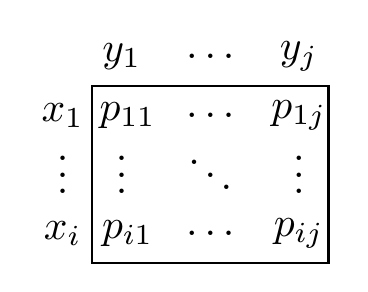
\begin{tikzpicture}[scale=1.5, every node/.style={transform shape}]
	\draw[thick] (0.5,0.5) -- (2.5,0.5) -- (2.5,2) -- (0.5,2) -- cycle;
	\draw (0.25,0.75) node {\(x_i\)};
	\draw (0.25,1.35) node {\(\vdots\)}; 
	\draw (0.25,1.75) node {\(x_1\)}; 
	\draw (0.75,2.25) node {\(y_1\)};
	\draw (1.5,2.25) node {\(\dots\)};
	\draw (2.25,2.25) node {\(y_j\)};
	\draw (0.8,1.75) node {\(p_{11}\)};
	\draw (0.8,0.75) node {\(p_{i1}\)};
	\draw (2.25,0.75) node {\(p_{ij}\)};
	\draw (2.25,1.75) node {\(p_{1j}\)};
	\draw (1.5,1.75) node {\(\dots\)};
	\draw (1.5,0.75) node {\(\dots\)};
	\draw (0.75,1.35) node {\(\vdots\)};
	\draw (2.25,1.35) node {\(\vdots\)};
	\draw (1.5,1.35) node {\(\ddots\)};
\end{tikzpicture}

	\caption[Schema Kontingenztabelle]{Schema einer Kontingenztabelle}
	\label{fig:contingency_ex}
\end{figure}

Multivariate Verteilungen beschreiben die Wahrscheinlichkeitsverteilung einer mehrdimensionalen Zufallsvariable bzw. mehrerer Zufallsvariablen. Zumindest für 2-dimensionale Zufallsvariablen kann die Verteilung in einer \textit{Kontingenztabelle} dargestellt werden, die schematisch in Abb.~\ref{fig:contingency_ex} zu sehen ist. Summiert man die einzelnen Spalten auf, so erhält man die Randverteilung für \(X\); summiert man die einzelnen Zeilen auf, so erhält man die Randverteilung von \(Y\).

Die Zufallsvariablen können aber auch voneinander abhängen. Die Verteilung einer Zufallsvariable, gegeben den Wert der anderen, nennt man \textbf{bedingte Verteilung} und wir durch
\[
	P(X=a\ |\ Y=b)=\frac{P(X=a,Y=b)}{P(Y=b)}
\]
beschrieben. Mithilfe der Kontingenztablle lassen sich die Werte des Bruchs direkt ablesen. Falls die Variablen \textbf{unabhängig} voneinander sind, gilt \(P(X) = P(X|Y)\) und \(P(X,Y) = P(X)P(Y)\).

Sei im Folgenden \(X\) eine diskrete Zufallsvariable. Dann bezeichnet \(f(x)=P(X=x)\) für alle \(x\in\mathbb{R}\) die Wahrscheinlichkeitsfunktion von \(X\). Für \(f(x)\) gilt \textit{Nichtnegativität} und es muss \(\sum f(x) = 1\) sein. Würde man diese Funktion plotten, so hätte man im Prinzip ein Stabdiagramm.
Sei \(X\) nun kontinuierlich. Damit ergibt sich die \textit{Wahrscheinlichkeitsdichtefunktion} zu \(P(X\in[a,b])=\int_{a}^{b} f(x)dx\) und auch hier gilt \textit{Nichtnegativität}. Weiter muss \(\int_{-\infty}^{\infty} f(x)dx = 1\) sein.

Der \textbf{Erwartungswert} \(E(X)\) für den diskreten bzw. kontinuierlichen Fall lautet
\begin{align*}
	&E(X)=\sum_{i\geq 1} x_i f(x_i) &E(X) = \int_{-\infty}^{\infty} xf(x)dx
\end{align*}
Durch den Verschiebungssatz erhalten wir für die \textbf{Varianz} \(Var(X)=E(X^2)-E(X)^2\). Somit ergeben sich für diskrete bzw. kontinuierliche Zufallsvariablen
\begin{align*}
	&Var(X)=\sum_i f(x_i) x_i^2 - (\sum_i f(x_i) \bar{x})^2 &Var(X)=\int_{-\infty}^{\infty} x^2f(x)dx - E(X)^2
\end{align*}

Um Zusammenhänge zwischen den Zufallsvariablen anschaulich darzustellen, gibt es bestimmte Kennzahlen. Zum einen die \textbf{Kovarianz}, die als
\begin{align*}
	Cov(X,Y) &:= E([X-E(X)][Y-E(Y)])\\
	\\
	Cov(X,Y) &= 
		\begin{cases}
		\sum\limits_i \sum\limits_j f(x_i,y_j)(x_i-E(X))(y_j-E(Y)) \hfill X \text{ und } Y \text{ diskret}\\
		\int\limits_{-\infty}^{\infty} \int\limits_{-\infty}^{\infty} f(x,y)(x-E(X))(y-E(Y))dxdy\quad X \text{ und } Y \text{ stetig}\\
		\end{cases}
\end{align*}
definiert ist. Betrachten wir die zweite Gleichung. In einem Koordinatensystem durch den Punkt \((E(X),E(Y))\) liefern die Werte des ersten und dritten Quadranten einen positiven Beitrag zur Gesamtsumme, die Werte des zweiten und vierten Quadranten hingegen negative. Damit ergibt sich, dass die Kovarianz zwar anzeigen kann, ob die Daten positiv/negativ korreliert sind oder unabhängig; da sie aber unskaliert ist, lässt sich die Stärke der Korrelation nicht sinnvoll qunatifizieren.
Eine gängige Normierung ergibt sich mittels der Standardabweichung und man erhält den \textbf{Korrelationskoeffizienten} 
\[
	\rho(X,Y) = \frac{Cov(X,Y)}{\sqrt{Var(X)} \sqrt{Var(Y)}}.
\] 
Dieser ist auf \([-1,1]\) normiert, womit sich nun auch die Stärke der Korrelation bewerten lassen kann. Des Weiteren gilt \(Cov(X,X)=Var(X)\).

Für den Fall, dass wir es mit einem Vektor an Zufallsvariablen zu tun haben, kommt die \textbf{Kovarianzmatrix} \(\Sigma\) ins Spiel. Die Kovarianzmatrix als Matrix aller paarweisen Kovarianzen der Elemente des Zufallsvektors enthält Informationen über seine Streuung und über Korrelationen ziwschen seinen Komponenten.
Formal ergibt sich:
\[
	\resizebox{\textwidth}{!}{
		\(\Sigma = (Cov(X_i,X_j))_{i,j = 1\dots n} = 
		\begin{pmatrix}
			Var(X_1) & Cov(X_1,X_2) &\dots & Cov(X_1,X_n)\\
			Cov(X_2,X_1)& Var(X_2) &\dots & Cov(X_2,X_n)\\
			\vdots &\vdots &\ddots &\vdots\\
			Cov(X_n,X_1) & Cov(X_n,X_2) &\dots &Var(X_n)
		\end{pmatrix}\)
	}
\] 

\subsection{Statistische Tests}
Die folgenden statistischen Tests sollen nur soweit vorgestellt werden, wie es nötig ist, sie anwenden zu können.
Für die genauen mathematischen Herleitungen und Zusammenhänge sei auf die entsprechende Fachliteratur verwiesen.

\subsubsection{Chi-Quadrat Unabhängigkeitstest}
\(\chi^{2}\)-Tests bezeichnen zunächst eine ganze Klasse von Tests. Hier wollen wir uns jedoch auf den Unabhängigkeitstest beschränken.
Mit ihm können wir eine Aussage über die Unabhängigkeit zweier Zufallsvariablen
 \(X\) und \(Y\) treffen. Meist liegt eine zu untersuchende Kontingenztabelle
vor. Damit lässt sich der gesamte Test kurz zusammenfassen:
\begin{itemize}
	\item \textbf{Annahmen:} Unabhängige  Stichprobenvariablen \((X_i,Y_i), i = 1,\dots , n\), gruppiert in eine \((k\times m)\)-Kontingenztabelle
	\item \textbf{Hypothese:} \begin{align*}
					&H_0: &P(X=i,Y=j) &= P(X=i) P(Y=j)\ \forall\ i,j\\
					&H_1: &P(X=i,Y=j) &\neq P(X=i) P(Y=j)\\
					& &\text{ für mindestens ein Paar } (i,j).&
				\end{align*}
	\item \textbf{Teststatistik:} \(\chi^2 =\sum\limits_{i=1}^{k}\sum\limits_{j=1}^{m}
					\frac{(h_{ij}-\tilde{h}_{ij})^2}{\tilde{h}_{ij}}\) mit \(\tilde{h}_{ij} = \frac{ h_{i\bullet} h_{\bullet j}}{ n } \)
	\item \textbf{Verteilung unter } \(H_0\): approximativ \(\chi^2((k-1)(m-1))\)
	\item \textbf{Ablehnungsbereich:} \(\chi^2 > \chi_{1-\alpha}^2((k-1)(m-1))\)
\end{itemize}
Der Verlust der Freiheitsgrade tritt durch die Schätzung \(\tilde{h}_{ij}\) auf.
Mit anderen Worten: Ist ein \(\chi^2\)-Wert besonders groß, so kann der entsprehcenden
Tabelle die Wahrscheinlichkeit für so einen Wert entnommen werden. Ist dieser sehr
klein, so wird die Nullhypothese verworfen. Bei diesem Test ist zu beachten,
dass der \(\chi^2\)-Wert in hohem Maße von dem Stichprobemumfang \(n\) abhängig ist.

\subsubsection{Kolmogorov-Smirnov-Test}
Dieser Test eignet sich, um Verteilungsannahmen zu prüfen. Es wird angenommen, 
dass die beobachteten Ereignisse bereits sortiert vorliegen. Aus diesen Werten
wird nun die Summenhäufigkeitsfunktion (empirische Verteilungfunktion) \(S\) berechnet,
die nun mit der angenommenen Verteilungsfunktion \(F_0\) verglichen wird. Hierfür werden
an den Stellen \(x_i\) die Differenzen der beiden Funktionen berechnet, also
\(S(x_{i-1}-F(x_i)\) und \(S(x_i)-F(x_i)\). Hierbei ist \(S(x_0):=0\). Man prüft also
die Stärke der Abweichung der angenommenen Funktion von den echten Werten.
Insgesamt ist damit also \(H_0:\ F(x)=F_0(x).\)
Die größte Differenz \(d_{max}\) wird nun mit den Tabellenwerten verglichen. 
Für \(n \leq 35\) liegen diese tabelliert vor, danach muss mit 
\(d_\alpha =\frac{\sqrt{-0,5\ln(\frac{\alpha}{2})}}{\sqrt{n}}\) approximiert werden.

Obwohl nur für eine Zufallsvariable formuliert, lässt sich der Test auch für 2 
Zufallsvariablen durchführen. Dabei gilt nun: \(H_0:\ F(y) = F(x)\).

\subsubsection{Wilcoxon-Mann-Whitney Test}
Auch bekant als Wilcoxon-Rangsummen-Test. Wir fassen kurz zusammen:
\begin{itemize}
	\item \textbf{Annahmen:} \(X_1,\dots,X_n\) unabhängige Wiederholungen von \(X\),\\
				\(Y_1,\dots,Y_m\) unabhängige Wiederholungen von \(Y\),\\
				\(X,Y\) sind unabhängig voneinander,\\
				die Verteilungsfunktionen unterscheiden sich nur durch eine Verschiebung \(a\) voneinander, also \(F_Y(x) = F_X(x-a)\). 
	\item \textbf{Hypothese:} \begin{align}
					&H_0: x_{med}=y_{med} 	&H_1: x_{med}\neq y_{med} \tag{a}\\
					&H_0: x_{med}\leq y_{med} &H_1: x_{med} > y_{med} \tag{b}\\
					&H_0: x_{med}\geq y_{med} &H_1: x_{med} < y_{med} \tag{c}
				\end{align}
	\item \textbf{Teststatistik:} Sortiere die Beobachtungen gepoolt und berechne die Summe der Ränge der
	Elemente der anfangs kleineren Strichprobe. Diese kleinere Stichprobe sei nun \(X\). Die Teststatistik ergibt sich damit als
	\(T_W = \sum\limits_{i=1}^n rg(X_i)\).
	\item \textbf{Ablehnungsbereich:} \begin{align}
						T_W &> w_{1-\alpha /2}(n,m) \text{ oder } T_W < w_{\alpha /2}(n,m) \tag{a}\\
						T_W &> w_{1-\alpha}(n,m) \tag{b}\\
						T_W &< w_{\alpha}(n,m) \tag{c}
					\end{align}
					wobei \(w_{\tilde{\alpha}}\) das \(\tilde{\alpha}\)-Quantil der tabellierten Verteilung bezeichnet.
\end{itemize}
Die genauen kritischen Werte lassen sich aus kombinatorischen Überlegungen 
berechnen. Diese werden jedoch schnell sehr mühselig zu berechnen, wodurch 
die Nutzung der Approximation durch
\[
	W_{n,m} \approx N \left( \frac{n(m+n+1)}{2}, \frac{nm(n+m+1)}{12} \right)
\]
ratsam ist. Die Idee, die hinter diesem Test steckt, ist, dass bei Gültigkeit
der Nullhypothese die Werte der \(X\)- und \(Y\)-Stichproben gut durchmischt
sein sollten, d.h. keine der beiden Stichproben zeigt im Verhältnis zur anderen
eine Tendenz zu besonders großen bzw. kleinen Werten. Der Test stellt nicht direkt
eine Gleichheit von zwei Verteilungen fest, sondern will lediglich eine Aussage über
die Mediane von \(X\) und \(Y\) treffen.

\subsubsection{Bernoulli-Experiment}
Sei \(n\) die Anzahl unserer Datenobjekte,
also die Anzahl der Versuche; \(p\) beschreibe nun die Erfolgswahrscheinlichkeit
eines einzelnen Experiments und \(S\) sei die Anzahl der erfolgreichen Experimente.
Damit ergibt sich als beobachtete Erfolgsquote \(f=\frac{S}{n}\). Ohne
Herleitung ist der Erwartungswert \(E(f) = p\) und die Varianz \(Var(f)= \frac{p(1-p)}{n}\).
Im Allgemeinen ist es das Ziel, \(p\) zu bestimmen, da dieses meist unbekannt ist.
Oft ist jedoch eher die Frage interessant, wie die Grenzen \(z\) gewählt werden
müssen, sodass 
\[
	P(-z \leq f \leq z) = c
\]
gilt. Normiert man \(f\), so kann man die Werte für \(z\) aus der Tabelle
der Standardnormalverteilung ablesen. Es ergibt sich
\[
	P(-z < \frac{f-p}{\sqrt{p(1-p)n}} < z) = c ,
\]
was nun nach Umformung nach \(p\) die Grenzen für dieses liefert. Hierbei
muss man beachten, dass \(n\) groß sein muss. Wie groß, da scheiden sich
die Geister.

Wiederholt man nun ein Bernoulli-Experiment beliebig oft, so lässt sich auch
die Wahrscheinlichkeit für eine bestimmte Folge von Ausgängen berechnen. Formal
ergibt sich
\[
	\prod\limits_{i=1}^{n} p^{y_i} (1-p)^{1-y_i}
\]
wobei \(y_i\) den Ausgang des \(i\)-ten Experiments bezeichnet und nur die Werte
\(0\) oder \(1\) annehmen kann. Das bedeutet, dass im Produkt am Ende pro Faktor
entweder \(p\) oder \(1-p\) steht. Da \(p\) jeodch meist unbekannt ist, kann man
stattdessen \(E(p) = \frac{\sum y_i}{n}\) verwenden, was im Prinzip ein 
\textit{Maximum-Likelihood-Schätzer} für \(p\) ist. Und da es egal ist, ob man,
wenn man \(p\) maximieren möchte, den obigen Ausdruck selbst, oder den Logarithmus
davon berechnet, ergibt sich stattdessen die \textbf{Log-Likelihood-Funktion}
\[
	\sum\limits_{i_1}^n y_i \log{p} + (1-y_i)\log(1-p).
\]
Auch hier gilt, dass pro Summand vom inneren Term nur ein Summand übrig bleibt.
Die Log-Likelihood-Funktion bietet den Vorteil, dass man nicht so viele Produkte
berechenen muss, und das aufsummieren schneller geht.


\subsection{Datenreduktion}
Da wir in unserer heutigen Zeit ein Unmenge an Daten sammeln, ist es zum Teil nicht
mehr möglich, die Daten roh zu verarbeiten bzw. zu analysieren. Deswegen kann es
nötig werden, die Daten irgendwie zu verkleinern. Die grundsätzlichen Methoden
hierfür sind
\begin{itemize}
	\item \textbf{Numerosity Reduction} - Die Reduzierung der Anzahl der Datenobjekte
	\item \textbf{Dimensionality Reduction} - Die Reduzierung der Anzahl der Attribute
	\item \textbf{Diskretisierung} - Die Vergröberung der Attributwerte
\end{itemize}
Im Folgenden werden wir die einzelnen Methoden etwas genauer betrachten.

\subsubsection{Numerosity Reduction}
Hier muss grundlegend zwischen zwei Arten von Verfahren unterschieden werden. Die
einen sind \textit{parametrische} Verfahren, die anderen \textit{nichtparametrische}.
Beim parametrischen Verfahren werden zunächst statistische Tests auf den Datenbestand
(oder nur einen Teil davon) angewandt, welche die Art der Verteilung liefern. Kann
man nun annehmen, dass die Verteilung des Datenbestandes der einer bekannten Verteilung
folgt, so braucht man sich lediglich die Parameter der bekannten Verteilung (z.B 
Mittelwert und Varianz bei einer Normalverteilung) merken. Dass dies eine enorme
Reduktion darstellt ist offensichtlich.

Die nichtparametrischen Verfahren treffen zunächst keinerlei Annahme über die
Verteilung der Werte des Datenbestandes. Methoden zur Reduktion umfassen hier
\textit{Histogramme, Sampling} und \textit{Clustering}. Histogramme wurden bereits
weiter oben besprochen. \textbf{Sampling} bedeutet, dass nur ein möglichst 
repräsentativer Ausschnitt des Datenbestandes verwendet wird. Dies kann die 
Komplexität mancher Analysealgorithmen erheblich reduzieren. \textbf{Clustering}
ist relativ selbsterklärend, setzt jedoch voraus, dass sich die Daten in Cluster
aufteilen lassen. So kann man jedes Cluster am Ende für sich betrachten und muss
nur die relevanten Clustereigenschaften, z.B. Anzahl der enthaltenen Datenobjekte,
lienare Summe, square sum, etc., speichern, aus denen man dann Werte wie die
Clustermitte oder -radius berechnen kann. Auf diese Methode wird in einem späteren
Kapitel näher eingegangen.

\subsubsection{Dimensionality Reduction}
\textbf{Feature Selection:} Man kann Attribute, die unnötig sind, auch einfach
weglassen. Dies setzt jedoch ein Wissen über die spzifische Domäne voraus. Hat
man dieses Wissen nicht, müssen andere Maßstäbe angesetzt werden, z.B. welche 
Attribute lassen sich relativ gut mit anderen Anttriubutwerten vorhersagen,
sprich wo liegt eine Abhängigkeit vor? Da es insgesamt \(2^d\) mögliche
Teilmengen von Attributen gibt (\(d\) ist die Mächtigkeit der Domain), 
können wir die Lösung oft nicht direkt explizit ausrechenen. Hier
müssen Heuristiken zur Auswahl der Dimensionen angewandt werden, z.B. wird zuerst die
\textit{Vorhersagekraft} jedes Attributs ermittelt und nur die besten Attribute
werden behalten, oder schrittweise Auswahl der miteinander am vorhersagekräftigsten
Attribute bis man genügend hat, oder eine schrittweise Eliminierung der am
wenigsten nützlichen Attribute.

\textbf{Hauptachsentransformation:} Auch Singulärwertzerlegung genannt, oder auf 
englisch Principal Component Analysis, Singular Value Decomposition oder Latent 
Semantic Indexing. Gegeben einem Datenbestand von \(N\) \(k\)-dimensionalen 
Datenobjekten: Finde nun \(c\leq k\) orthogonale Vektoren, die den Datenbestand
am besten repräsentieren. Lägen beispielsweise alle Datenpunkte im \(\mathbb{R}^2\)
auf einer Geraden durch den Ursprung, so würde es sich doch anbieten, die Gerade
als neue Hauptachse zu nehmen und die andere Achse wegzulassen, da mit der Geraden
bereits alle Datenobjekte beschrieben werden. Dieser Fall ist natürlich komplett
konstruiert; würden sich aber die Werte relativ nah um eine Gerade herum verteilen,
so würde diese Gerade schon ausreichen.

Diese eher graphische Darstellung kann mit der Singulärwertzerlegung auch für
Matrizen und höher-dimensionale Probleme angewandt werden. Da SVD eine äußerst
wichtige Methode zur Datenreduktion und auch Analyse ist, wollen wir hier mit 
einem extensiveren Beispiel arbeiten, als es in der Vorlesung gegeben ist.

% latex table generated in R 3.2.3 by xtable 1.8-2 package
% Sun Nov  6 23:03:19 2016
\begin{table}[th]
	\centering
	\caption{Ein Beispiel Datenbestand mit Filmbewertungen von verschieden Personen.}
	\label{tab:svd_example}
	\resizebox{\textwidth}{!}{
\begin{tabular}{rrrrrrr}
  \hline
 & Avengers & Dr.Strange & Ant.Man & Batman & Superman & Watchmen \\ 
  \hline
Tony &  10 &   9 &   8 &   1 &   0 &   0 \\ 
  Thor &  10 &  10 &   7 &   0 &   0 &   1 \\ 
  Stephen &   8 &  10 &   8 &   0 &   0 &   0 \\ 
  Scott &  10 &   9 &  10 &   2 &   0 &   0 \\ 
  Bruce &   1 &   0 &   0 &  10 &   9 &   8 \\ 
  Clark &   2 &   0 &   0 &   9 &  10 &   9 \\ 
  Dr. Manhatten &   1 &   0 &   0 &   7 &   7 &  10 \\ 
  Rorschach &   0 &   0 &   0 &   9 &   8 &  10 \\ 
   \hline
\end{tabular}
}
\end{table}


Betrachten wir also zunächst Tablle~\ref{tab:svd_example}. Man kann durchaus vermuten,
dass die jeweiligen Superhelden die Filme aus ihrem eigenen Universum besser bewerten.
Diese Werte lassen sich auch in Form einer Matrix \(A\) aufschreiben

\begin{align*}
	A = % latex table generated in R 3.2.3 by xtable 1.8-2 package
% Sun Nov  6 23:25:21 2016
\begin{bmatrix}{}
   10 &   9 &   8 &   1 &   0 &   0 \\ 
   10 &  10 &   7 &   0 &   0 &   1 \\ 
    8 &  10 &   8 &   0 &   0 &   0 \\ 
   10 &   9 &  10 &   2 &   0 &   0 \\ 
    1 &   0 &   0 &  10 &   9 &   8 \\ 
    2 &   0 &   0 &   9 &  10 &   9 \\ 
    1 &   0 &   0 &   7 &   7 &  10 \\ 
    0 &   0 &   0 &   9 &   8 &  10 \\ 
  \end{bmatrix}

\end{align*}
Für diese \(m\times n\)-Matrix \(A\) mit Rang \(r\) gilt nun, dass sie sich immer 
Zerlegen lässt in
\[
	A = U\Sigma V^*
\]
wobei \(U\) eine \textbf{unitäre} \(m\times m\)-Matrix\footnote{\textbf{Unitär} bedeutet,
dass \(U^{H}*U = I\), wobei \(U^{H}\) die Adjungierte ist.}, \(\Sigma\) eine 
reelle \(m\times n\)-Matrix und \(V^*\) die \textbf{Adjungierte}\footnote{
\textbf{Adjungiert} ist die komplex-kunjugierte Transponierte einer Matrix (die Reihenfolge der
Operationen ist hierbei unerheblich).} einer
\textbf{unitären} \(n\times n\) Matrix \(V\) ist. \(\Sigma\) hat die spezielle Form, dass
sich auf den ersten \(r\) Diagonaleneinträgen die \textbf{Singulärwerte}\footnote{Singulärwerte
können als Streckung der Vektoren betrachtet werden.} von \(A\)
befinden, die auch durch \(A\) eindeutig bestimmt sind. Alle anderen Werte von
\(\Sigma\) sind \(0\). Die Spaltenvektoren von \(U\) heißen \textbf{Links-Singulärvektoren}
und die Spaltenvektoren von \(V\) heißen \textbf{Rechts-Singulärvektoren}.
Das scheint erstmal wieder schrecklich viel Mathe zu werden. Es sollen aber im
Endeffekt zunächst nur die Begriffe hängen bleiben. Fahren wir mit dem Anschaulichen
fort. Lassen wir uns die Werte aus Tabelle~\ref{tab:svd_example} in einer Heatmap
plotten, ergibt sich Abb.~\ref{fig:original_data}.

\begin{figure}[!th]
	\center
	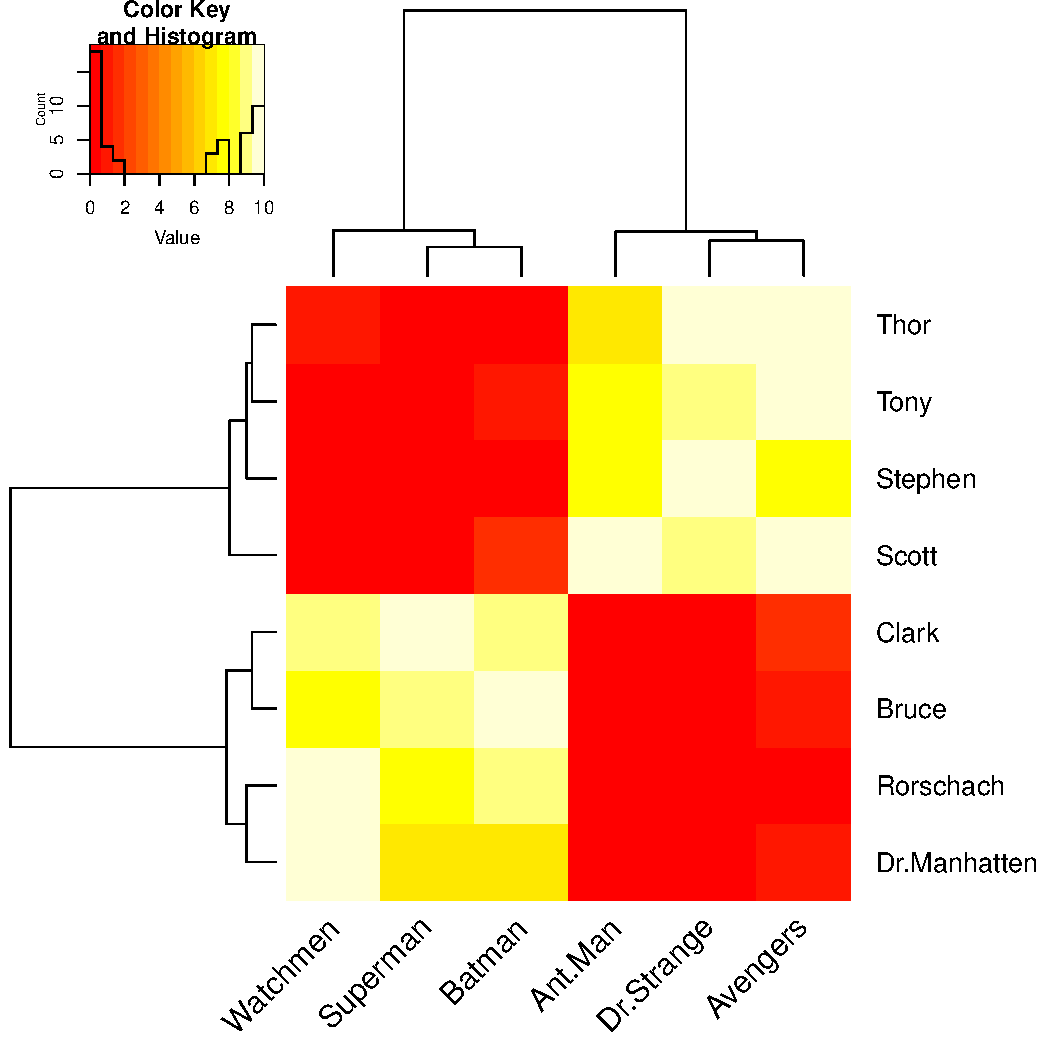
\includegraphics[width=0.5\textwidth]{Figures/original_data}
	\caption{Die Rohdaten als Heatmap.}
	\label{fig:original_data}
\end{figure}

Aus dieser Heatmap lässt sich einfach erkennen, dass es offensichtlich zwei
Cluster gibt, nämlich die Marvel-Fans und die DC-Fans, welche die jeweils anderen
hassen. Es gibt also zwei "'Konzepte"', die den Datenbestand prägen. Damit kann
es also durchaus interessant sein, die Anzahl der betrachteten Dimensionen auf ein
Minimum zu reduzieren, ohne einen großen Informationsverlust in Kauf nehmen zu müssen.
Hierfür ist die Singulärwertzerlegung zuständig. Wendet man in \textit{R} auf
obigen Datenbestand die \textit{svd()}-Funktion an, so ergibt sich

\begin{align*}
	U &= % latex table generated in R 3.2.3 by xtable 1.8-2 package
% Mon Nov  7 00:01:39 2016
\begin{bmatrix}{}
  -0.41 & 0.28 & -0.11 & -0.14 & -0.31 & 0.22 \\ 
  -0.41 & 0.28 & 0.43 & -0.44 & -0.07 & 0.36 \\ 
  -0.38 & 0.29 & 0.16 & 0.09 & 0.75 & -0.36 \\ 
  -0.44 & 0.29 & -0.43 & 0.50 & -0.31 & -0.19 \\ 
  -0.29 & -0.41 & -0.47 & -0.14 & 0.26 & 0.46 \\ 
  -0.32 & -0.42 & -0.18 & -0.51 & -0.11 & -0.59 \\ 
  -0.26 & -0.37 & 0.55 & 0.26 & -0.35 & -0.16 \\ 
  -0.28 & -0.43 & 0.18 & 0.43 & 0.21 & 0.28 \\ 
  \end{bmatrix}
\\
	\Sigma &= % latex table generated in R 3.2.3 by xtable 1.8-2 package
% Mon Nov  7 00:01:39 2016
\begin{bmatrix}{}
  32.43 & 0.00 & 0.00 & 0.00 & 0.00 & 0.00 \\ 
  0.00 & 29.87 & 0.00 & 0.00 & 0.00 & 0.00 \\ 
  0.00 & 0.00 & 3.36 & 0.00 & 0.00 & 0.00 \\ 
  0.00 & 0.00 & 0.00 & 2.32 & 0.00 & 0.00 \\ 
  0.00 & 0.00 & 0.00 & 0.00 & 1.82 & 0.00 \\ 
  0.00 & 0.00 & 0.00 & 0.00 & 0.00 & 1.01 \\ 
  \end{bmatrix}
\\
	V &= % latex table generated in R 3.2.3 by xtable 1.8-2 package
% Mon Nov  7 00:00:14 2016
\begin{bmatrix}{}
  -0.52 & 0.31 & -0.04 & -0.44 & -0.65 & 0.13 \\ 
  -0.48 & 0.37 & 0.30 & -0.13 & 0.68 & 0.26 \\ 
  -0.42 & 0.32 & -0.27 & 0.64 & -0.03 & -0.49 \\ 
  -0.35 & -0.45 & -0.53 & 0.22 & 0.06 & 0.58 \\ 
  -0.30 & -0.47 & -0.21 & -0.49 & 0.25 & -0.58 \\ 
  -0.34 & -0.50 & 0.71 & 0.30 & -0.22 & -0.03 \\ 
  \end{bmatrix}

\end{align*}

Wenn wir uns nun \(\Sigma\) etwas näher anschauen, stellen wir fest, dass es
zwei große Werte gibt, nämlich \(\sigma_1\) und \(\sigma_2\), und die anderen
Werte eher schwach ausfallen. Dies zeigt uns, dass die einzigen wirklich aussagekräftigen
Werte \(\sigma_1\) und \(\sigma_2\) sind und wir die übrigen vernachlässigen
können. Dies geschieht, indem alle anderen \(\sigma\) gleich \(0\) gesetzt werden,
wodurch bei der Multiplikation \(U\Sigma V^*\) die rechten Spalten von \(U\) und die
unteren Zeilen von \(V^*\) effektiv wegfallen.
Am Ende kommt eine Art Approxmination \(\tilde{A}\) von \(A\) heraus mit
\[
	\tilde{A} = % latex table generated in R 3.2.3 by xtable 1.8-2 package
% Mon Nov  7 01:11:22 2016
\begin{bmatrix}{}
  9.45 & 9.39 & 8.20 & 0.78 & 0.03 & 0.25 \\ 
  9.47 & 9.42 & 8.22 & 0.79 & 0.04 & 0.26 \\ 
  9.04 & 9.03 & 7.88 & 0.37 & -0.34 & -0.16 \\ 
  10.12 & 10.03 & 8.75 & 1.11 & 0.30 & 0.56 \\ 
  1.04 & -0.01 & 0.02 & 8.92 & 8.66 & 9.34 \\ 
  1.40 & 0.31 & 0.29 & 9.30 & 9.00 & 9.71 \\ 
  0.94 & -0.00 & 0.02 & 7.99 & 7.75 & 8.36 \\ 
  0.67 & -0.38 & -0.31 & 8.92 & 8.69 & 9.36 \\ 
  \end{bmatrix}

\]
Wie man sehen kann, sind die Werte dieser Approximation relativ nahe an den
echten Werten von \(A\) dran.

\begin{figure}[!th]
	\center
	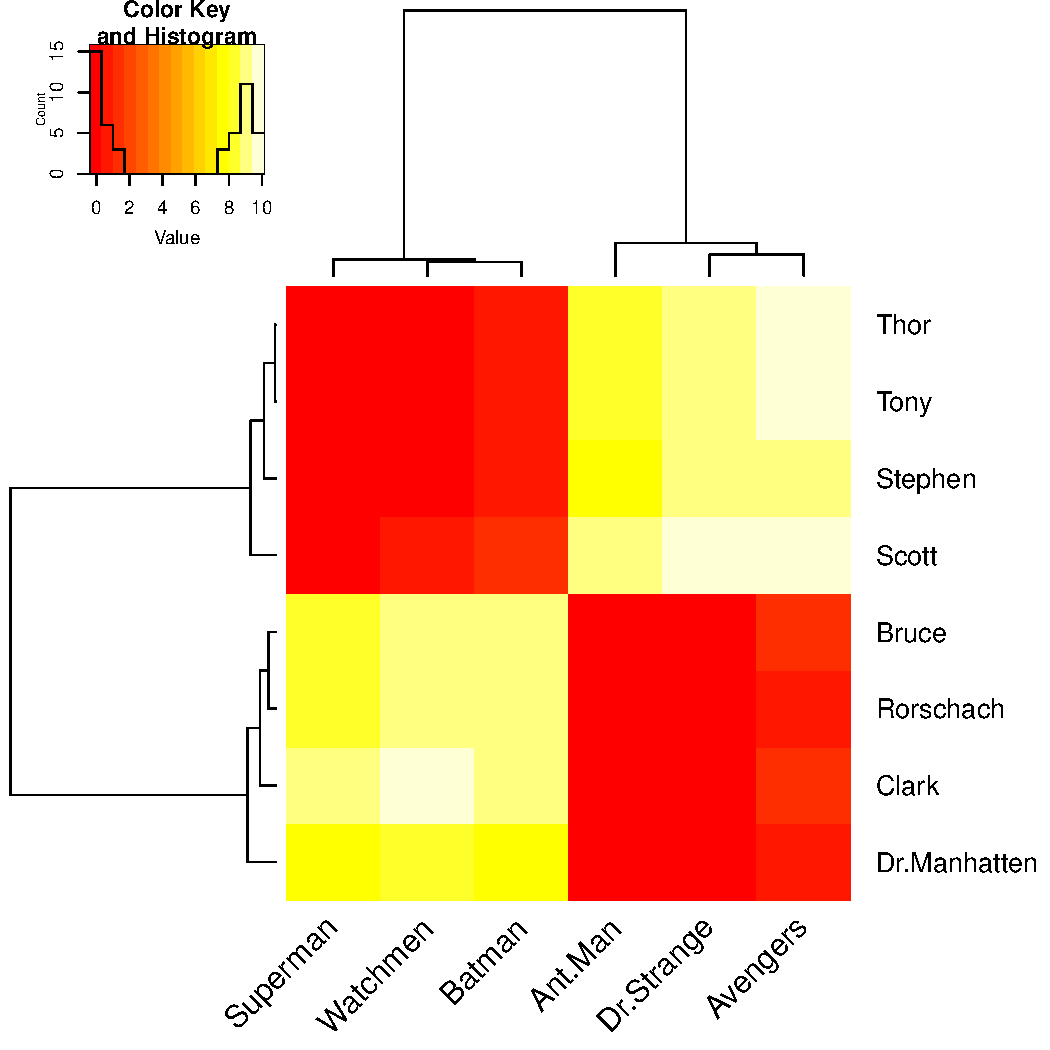
\includegraphics[width=0.5\textwidth]{Figures/reduced_data}
	\caption{Die Heatmap für die Approximation mit reduzierten Daten.}
	\label{fig:reduced_data}
\end{figure}

Die Heatmap in Bild~\ref{fig:reduced_data} zeigt, dass durch die Singulärwertzerlegung
die Struktur der Daten weitestgehend erhalten geblieben ist.

Es sei an dieser Stelle ein Wort der Warnung gegeben: Sollten weitere Datensätze
hinzukommen, die sich nicht so einfach den einzelnen Clustern zuordnen lassen,
wie z.B. die Gottheiten aus Lovecrafts Geschichten, die weder an Marvel noch an DC
besonderen Gefallen finden, so wird die Interpretation der erhaltenen Matrizen
sehr schnell schwierig und die Werte für die Singulärwerte sind auch weitaus weniger
eindeutig. Es ist also im Allgemeinen nicht so einfach, passende Werte zu finden,
die die Struktur des Datenbestanden treffend wiedergeben.

\subsubsection{Diskretisierung}
Okay, wir halten uns kurz.  \textbf{Entropiebasierte Diskretisierung:} Wir teilen
unseren Datenbestand \(S\) auf in kleinere Partitionierungen. Wo genau wir aber
die Intervallsgrenzen am besten setzen, verrät uns die \textbf{Entropie des Splits}:
\[
	Entropie_{Split}(S,T) = \frac{|S_1|}{|S|} Entropie(S_1) +
	\frac{|S_2|}{|S|} Entropie(S_2)
\]
Hierbei ist \(T\) der Schwellenwert für den Split. Diesen gilt es effizient zu wählen.
Natürlich lässt sich das auch für mehr als 2 Partitionen machen. Optimal ist unsere
Partitionierung, wenn obige Funktion minimiert wird. Die Berechnung wird rekursiv
durchgeführt, bis irgendein Abbruchkriterium erfüllt ist.

Grundsätzlich kann man zwischen \textit{top-down} und \textit{bottom-up} Verfahren
bei der Diskretisierung unterscheiden, die dann entweder Split- oder Merge-basiert
arbeiten. Hat man z.B. bereits eine Partitionierung kleinen Intervalls, hat jedoch
zu viele Partitionen, ist es sinnvoll, gut zusammenpassende Intervalle zu einem
größere zusammenzufassen. Ein passender Algorithmus wäre der s.g. \textbf{Chi-Merge},
der darauf beruht, dass der \(\chi^2\)-Test auf den einzelnen Intervallen 
Zusammenhänge zwischen den Verteilungen der Intervallnachbarn aufdeckt, und diese
bei Übereinstimmung zusammenfügt. Dieser Algorithmus läuft ebenfalls so lange,
bis irgendein Abbruchkriterium erfüllt ist. Wir werden nicht näher auf ihn
eingehen, \texttt{R} und andere Statistik Software können das auch so berechnen.
